\documentclass[aspectratio=169]{beamer}
\usepackage[utf8]{inputenc}
\usepackage{graphicx}
\usepackage{minted}
\usepackage{listings}
\usepackage{xcolor}
\definecolor{codecolor}{HTML}{FFC300}
\let\textttorig\texttt
\renewcommand<>{\texttt}[1]{%
  \only#2{\textttorig{#1}}%
}
\usepackage{hyperref}
\DeclareUrlCommand\url{\color{blue}}
\usetheme[sidebarleft]{Caltech}
\title[Linear Algebra]
{\bfseries{SSA Linear Algebra Final}}
\subtitle{Image Convolution in MATLAB (and a bit of Python)}
\author[FINAL EXAM]
{Evan Xiang\inst{1} \and Vivan Poddar\inst{1} \and Rohan Khera\inst{1} \and Beau Brush\inst{1}}
\institute[Caltech]
{
  \inst{1}
  Mathematics Department\\
  Shady Side Academy Senior School
}
\date[ICUP, 2014]
{\\December 16th, 2024}
\begin{document}
\frame{\titlepage}  

\begin{frame}
\frametitle{Table of Contents}
\tableofcontents
\end{frame}

\section{Overview}
\begin{frame}
\frametitle{Convolution Overview}
\begin{block}{Definition}
A convolution is done by multiplying a pixel’s and its neighboring pixels color value by a matrix.
\end{block}
\begin{block}{Generalized Matrix Convolution Formula}
$$(F * G)(x, y) = \sum_{m} \sum_{n} F(x - m, y - n) G(m, n)
$$
Where:
\begin{itemize}
    \item $x$ and $y$ represent the current position within the output matrix
    \item $m$ and $n$ are generalized variables representing the shift of the matrix with regard to $G(m,n) \rightarrow$  the kernel matrix
\end{itemize}
\end{block}
\end{frame}
%---------------------------------------------------------
\begin{frame}
\frametitle{Convolution Cont.}
\begin{columns}
\column{0.45\textwidth}
\begin{figure}
    \centering
    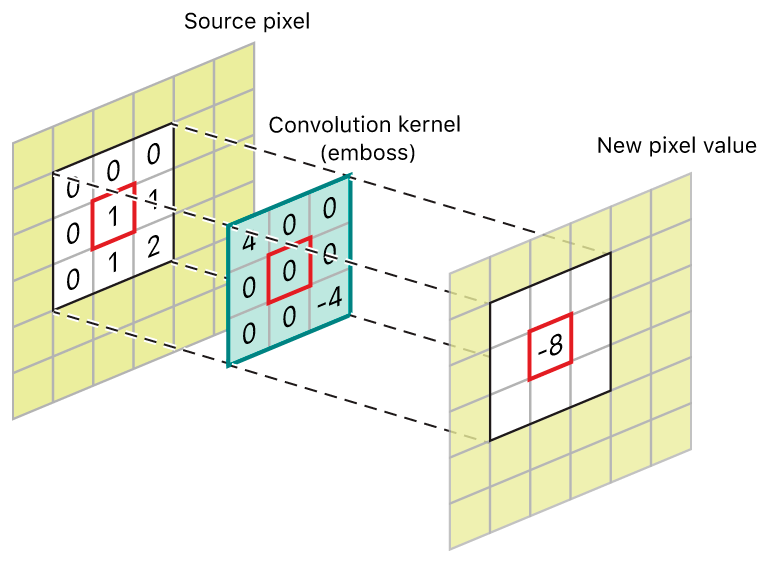
\includegraphics[width=\columnwidth]{figures/convolution.png}
    \caption{A general description of the convolution operation. \tiny{(Photo downloaded from Apple Developer Documentation, CC BY-SA 4.0)}}
    \label{fig:convolution}
\end{figure}

\column{0.55\textwidth}
\begin{block}{Summary of the Convolution Operation}
\begin{itemize}
\scriptsize
\item Place the kernel \(G(m, n)\) over the input matrix \(F(x, y)\) such that the kernel's center aligns with the current position \((x, y)\) of the output matrix.
\item For every element of the kernel \(G(m, n)\), multiply it with the corresponding element of the input matrix \(F(x - m, y - n)\).
\item Sum all the resulting products to compute the value for the current position \((x, y)\) in the output matrix.
\[
(F * G)(x, y) = \sum_m \sum_n F(x - m, y - n) G(m, n)
\]
\item Slide the kernel over the input matrix to the next position and repeat steps 2 and 3. This involves systematically shifting the kernel across all valid positions in the input matrix.

\end{itemize}
\end{block}
\end{columns}
\end{frame}

%---------------------------------------------------------
\section{Gaussian}
\begin{frame}
\frametitle{Weierstrass Transform (Gaussian Filter)}

\begin{columns}

\column{0.3\textwidth}

\begin{figure}
    \centering
    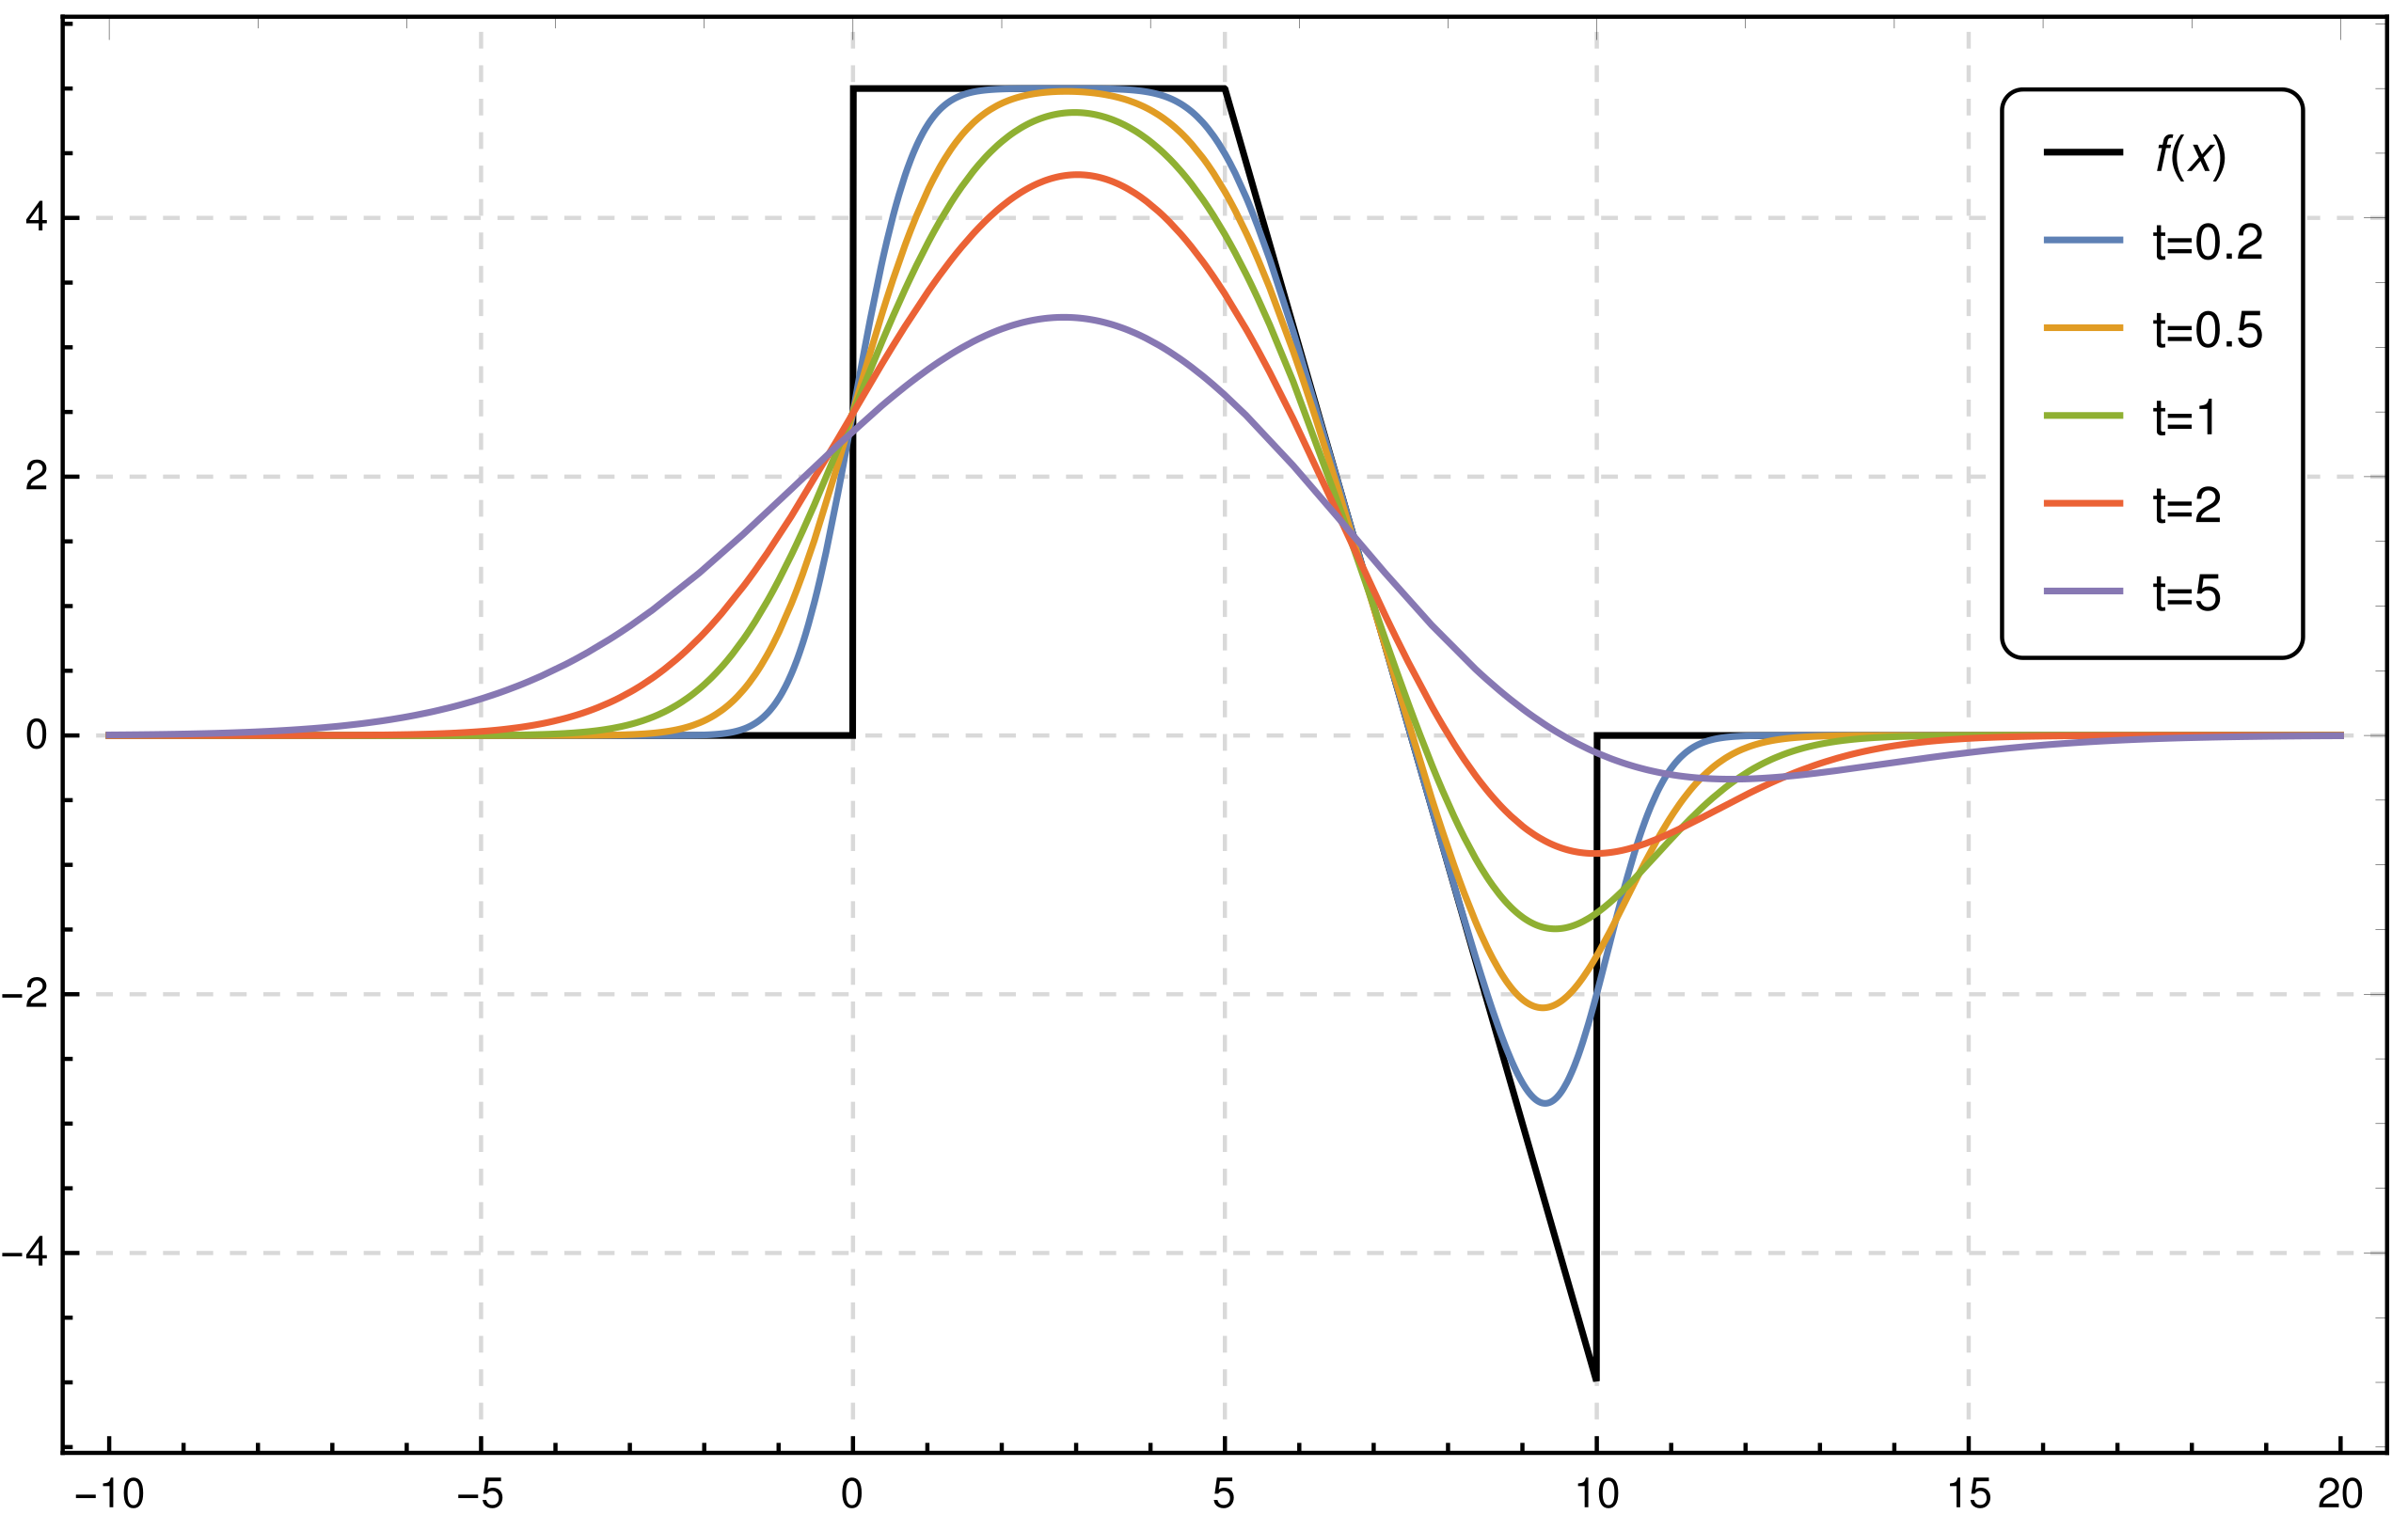
\includegraphics[width=\columnwidth]{figures/weierstrass.png}
    \caption{Weierstrass Transform for 5 parameters of $t$. The green line represents the standard Weierstrass. \tiny{(Photo downloaded from Glosser.ca - Own work, CC BY-SA 4.0)}}
    \label{fig:hollywood_prank}
\end{figure}
\column{0.7\textwidth}
\begin{block}{Definition}
The Weierstrass transform applies a 2D Gaussian Kernel to an image to reduce noise and create a blurred version of the original function by taking a weighted average of the function's values with the degree of smoothing controlled by the Gaussian's variance. 
\end{block}
\end{columns}
\end{frame}

\begin{frame}{Gaussian Cont.}
\begin{block}{Formula}
$$O(i, j) = \sum_{x=-\lfloor N/2 \rfloor}^{\lfloor N/2 \rfloor} \sum_{y=-\lfloor N/2 \rfloor}^{\lfloor N/2 \rfloor} \left( \frac{1}{2\pi\sigma^2} e^{-\frac{x^2 + y^2}{2\sigma^2}} \right) \cdot I(i-x, j-y)$$
Where:
\begin{itemize}
    \item $N$ represents the size of the kernel 
    \item $( \frac{1}{2\pi\sigma^2} e^{-\frac{x^2 + y^2}{2\sigma^2}})$ represents the Gaussian kernel
    \item $O(i,j)$ represents the output
\end{itemize}
\end{block}    
\end{frame}
%-----------------------------------------------------
\section{Cauchy}
\begin{frame}{Cauchy Kernel}
\begin{block}{Cauchy Matrix Convolution Formula}
$$O(i, j) = \sum_{x=-\lfloor N/2 \rfloor}^{\lfloor N/2 \rfloor} \sum_{y=-\lfloor N/2 \rfloor}^{\lfloor N/2 \rfloor} 
\frac{1}{\pi \gamma \left(1 + \frac{x^2 + y^2}{\gamma^2}\right)} \cdot I(i-x, j-y)
$$

Note that this looks relatively similar to the Weierstrass Transform with the Gaussian! But how does it differ...
\end{block}
\begin{block} {Gaussian vs. Cauchy Kernel}
The primary difference arises in the difference in the kernel decay rate. The Gaussian, represented by $K_{\text{Gaussian}}(r) = \exp\left(-\frac{r^2}{2\sigma^2}\right)$, decreases exponentially. The Cauchy, represented by $K_{\text{Cauchy}}(r) = \frac{\gamma}{\pi (\gamma^2 + r^2)}
$, decreases algebraically, allowing for longer distance influences. 
\end{block}
\end{frame}
%-----------------------
\section{Box Blur}
\begin{frame} {Box Blur Method}
\begin{block} {Formula}
    $$O(i, j) = \frac{1}{N^2} \sum_{x=-\lfloor N/2 \rfloor}^{\lfloor N/2 \rfloor} \sum_{y=-\lfloor N/2 \rfloor}^{\lfloor N/2 \rfloor} I(i-x, j-y)$$
    See how this is much simpler than all the previous algorithms... There's a reason for this... I mean it's literally just a weighted average of the values covered by the kernel applied to all values in the image matrix.
\end{block}
\end{frame}

\begin{frame}{The Gaussian in Disguise}
\begin{block} {Proof}
\footnotesize
The box blur operation is a convolution of the image \(I\) with \( K(x, y) \), producing a blurred output \( O(x, y) \). Repeated application of the box blur corresponds to convolving \( K(x, y) \) with itself \( n \) times. After \( n \) convolutions, the resulting kernel \( K_n(x, y) \) is given by:

\[
K_n(x, y) = K(x, y) * K(x, y) * \dots * K(x, y) \quad \text{(n times)}.
\]

By the Central Limit Theorem, the sum of \( n \) independent random variables converges to a Gaussian distribution as \( n \to \infty \) with finite mean and variance. The kernel \( K(x, y) \) acts as a probability distribution. Since the uniform box kernel \( K(x, y) \) satisfies the conditions of the CLT, the repeated convolution \( K_n(x, y) \) converges to a Gaussian kernel \( G(x, y) \):

\[
G(x, y) = \frac{1}{2\pi\sigma^2} \exp\left(-\frac{x^2 + y^2}{2\sigma^2}\right),
\]

where the standard deviation \( \sigma \) grows proportionally to \( \sqrt{n} \).

Thus, repeated application of the box blur approximates the Gaussian Kernel as \( n \to \infty \).
\end{block}
\end{frame}







\section{Kernel Implementation}

%---------------------------------------------------------
\begin{frame}{Kernel Implementation}
    \begin{figure}
        \centering
        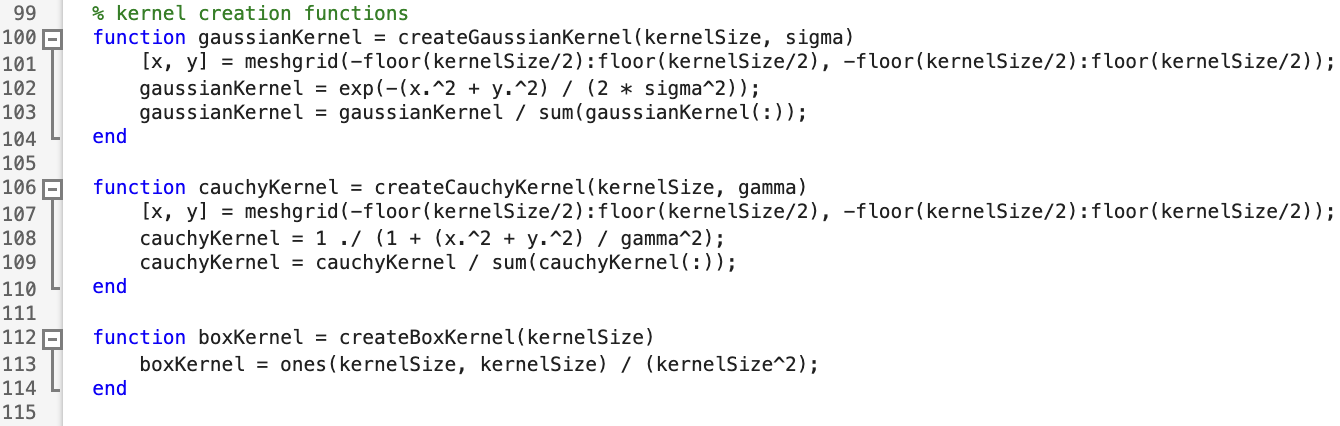
\includegraphics[width=\columnwidth]{figures/kernelcode.png}
        \caption{Implementation of all 3 kernels in MATLAB (.mat) code. Each function defines a separate type of kernel which can be called to slide across the pixels of an image.}
        \label{fig:kernelcode}
    \end{figure}
\end{frame}
\section{Sliding Window}
\begin{frame}{Sliding Window}
\begin{figure}
    \centering
    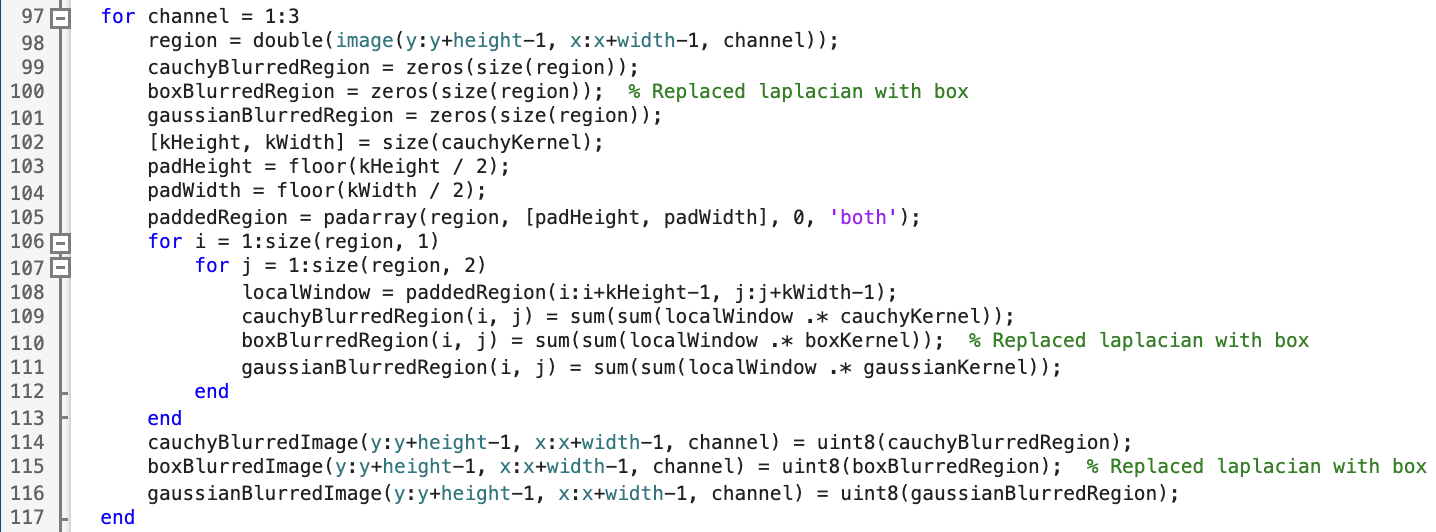
\includegraphics[width=1\linewidth]{figures/convolutioncode.png}
    \caption{Implementation of the full convolution operation, using the 3 separate kernels defined in the previous slide.}
    \label{fig:convcode}
\end{figure}
\end{frame}
\section{Interface}
\begin{frame}{Final Developed Interface}
\begin{figure}
    \centering
    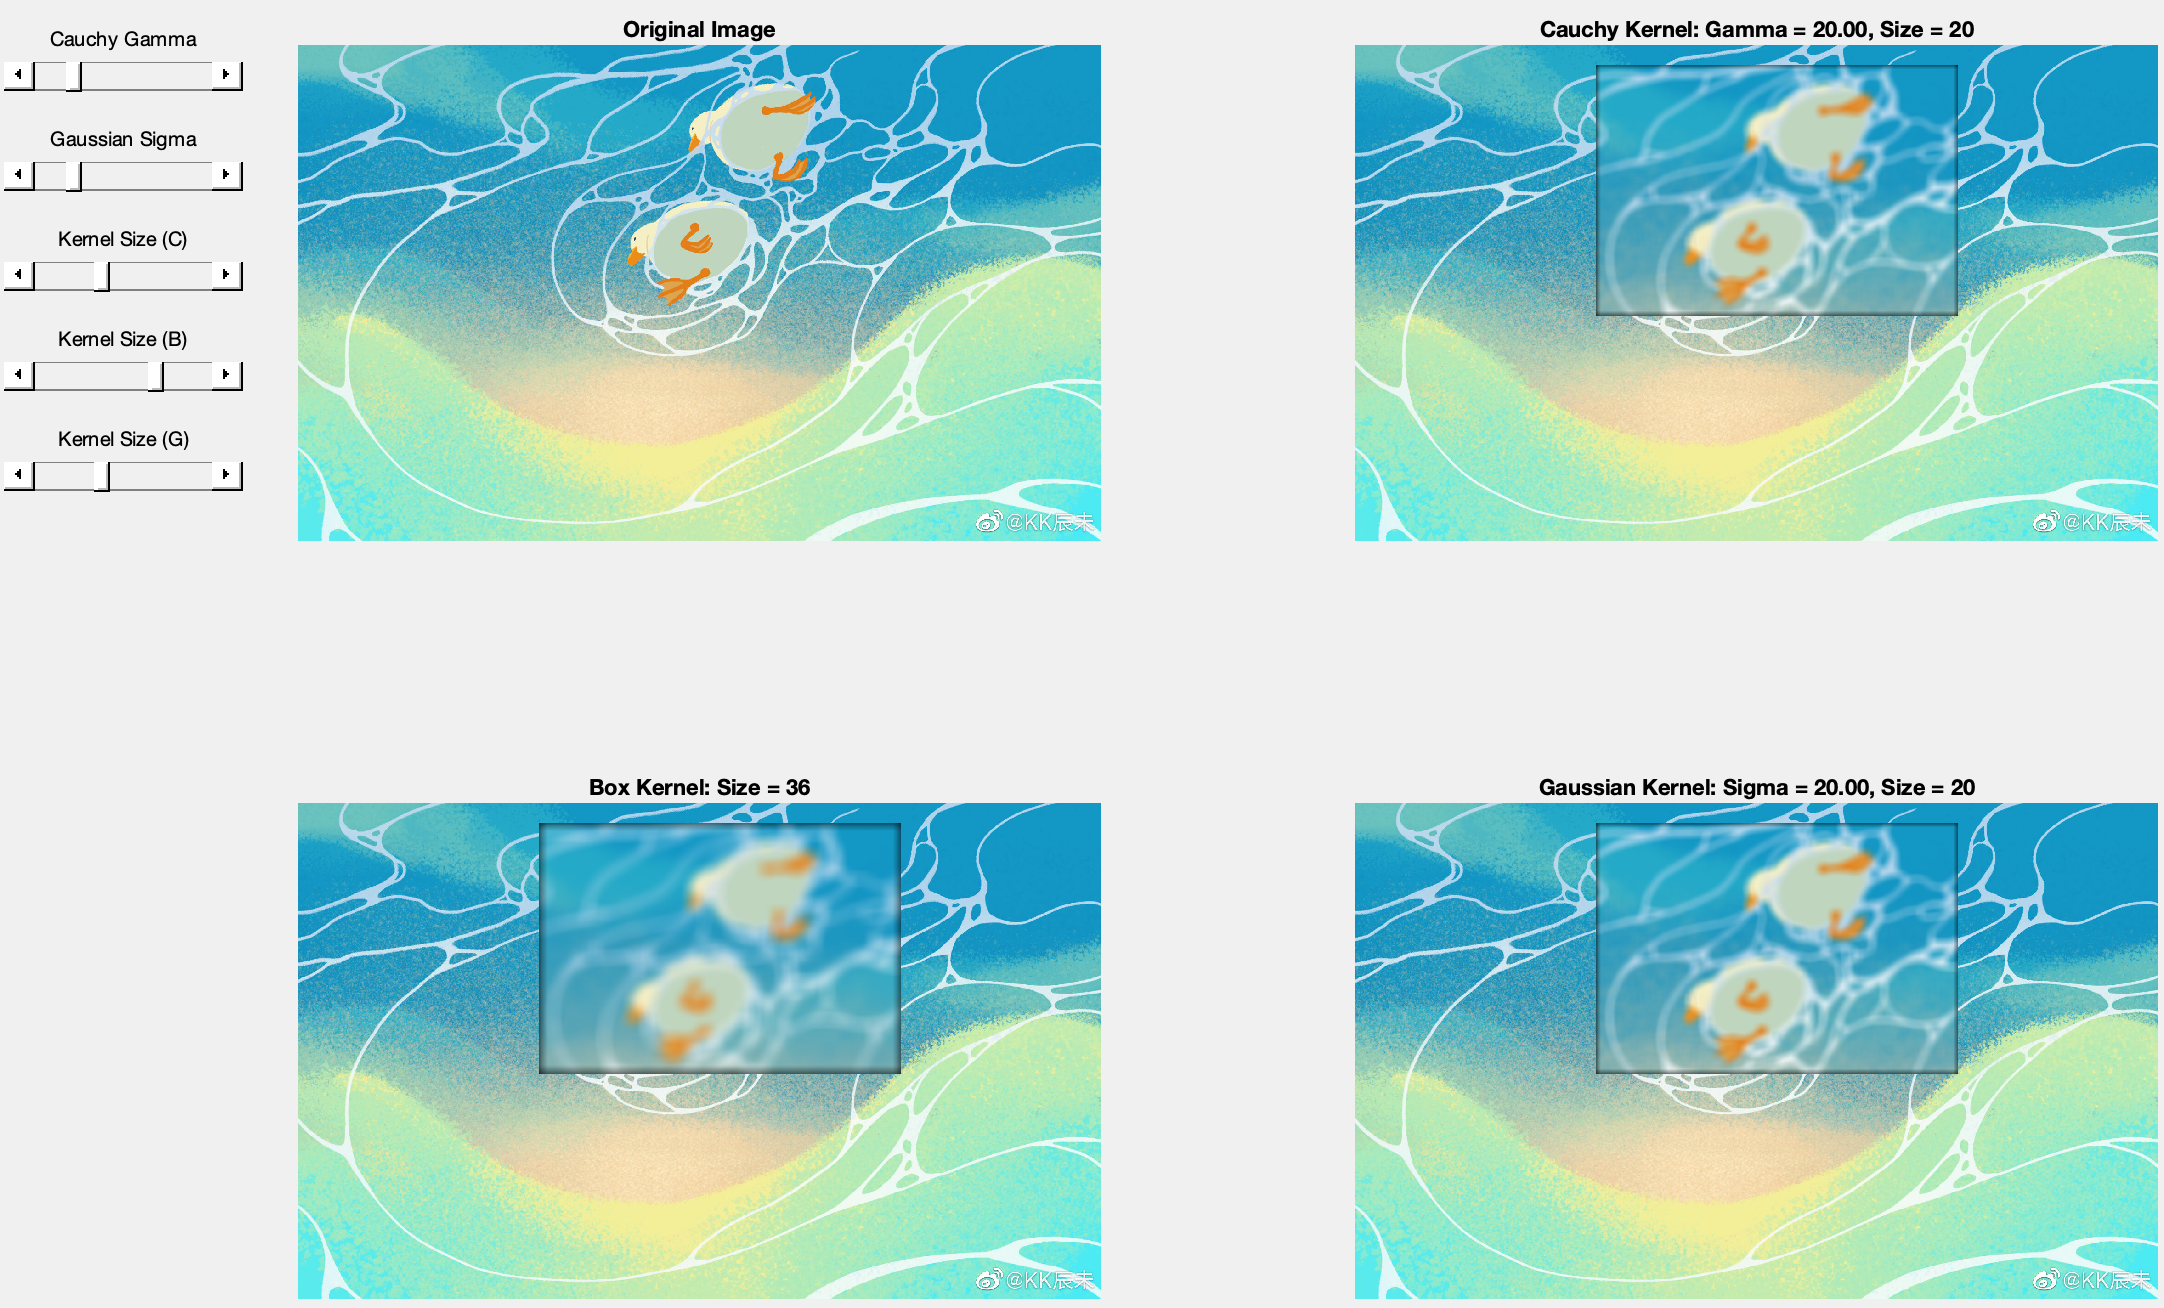
\includegraphics[width=0.9\linewidth]{figures/interface.png}
    \label{fig:interface}
\end{figure}
\end{frame}
\section{Proof}
\begin{frame}{Quod erat demonstrandum!}
\begin{figure}
    \centering
    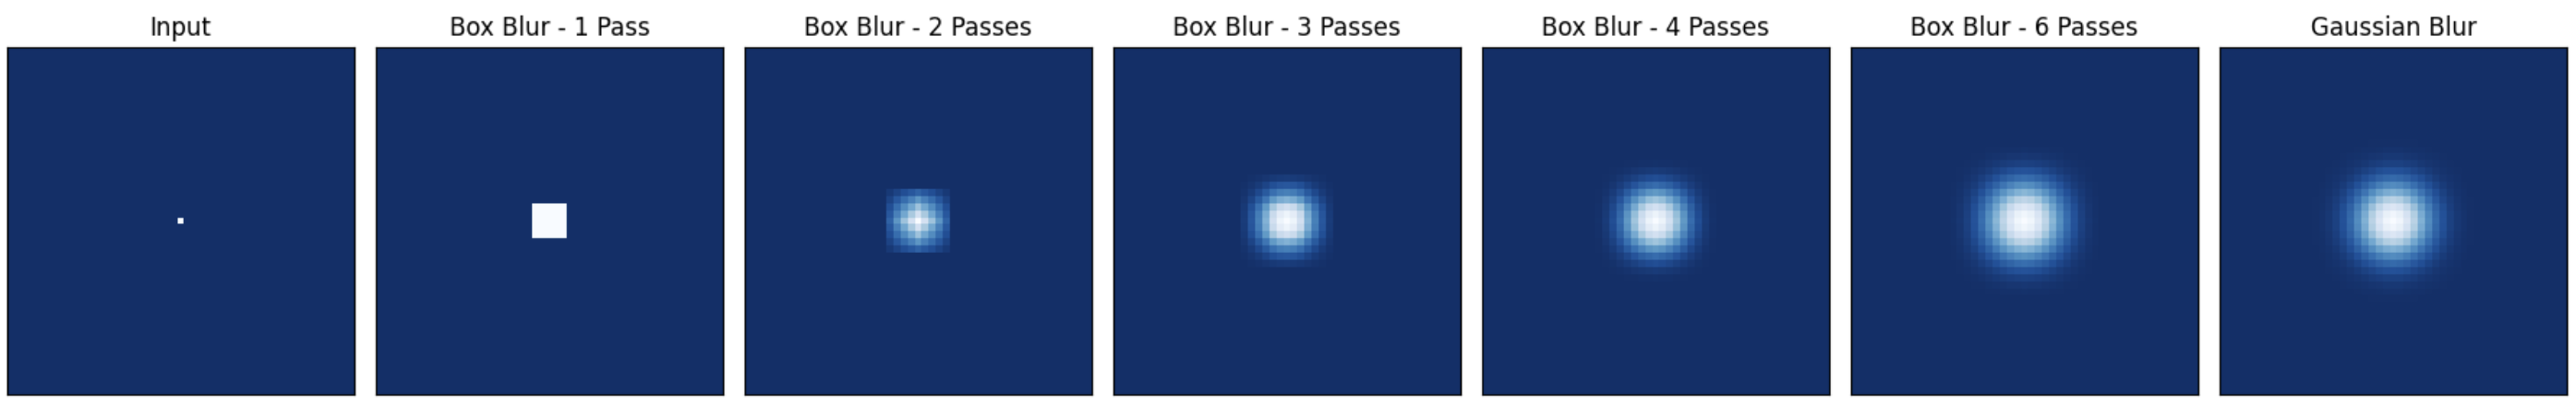
\includegraphics[width=1\linewidth]{figures/proof.png}
    \label{fig:proof}
\end{figure}
\vspace{-20pt}
\begin{figure}
    \centering
    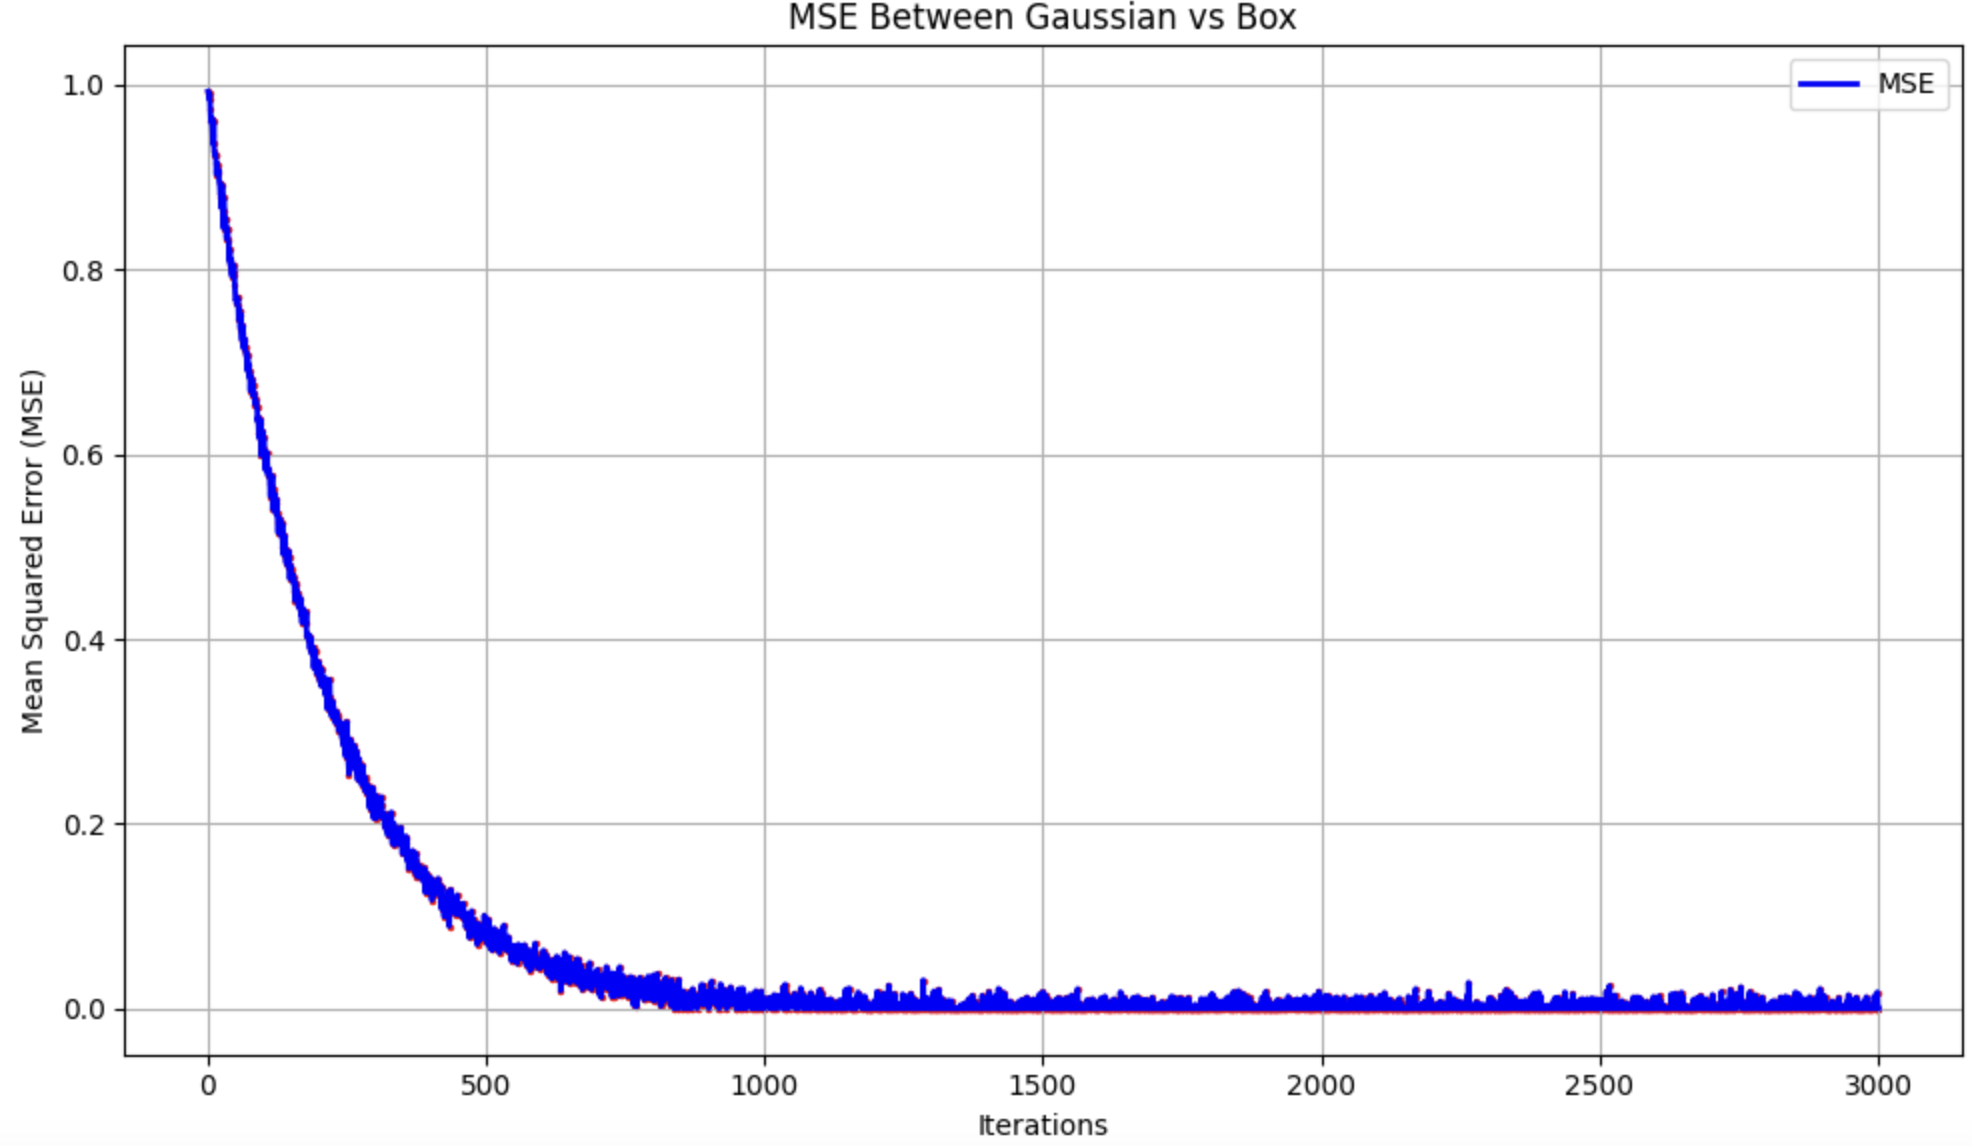
\includegraphics[width=0.6\linewidth]{figures/MSE.png}
    \label{fig:mse}
\end{figure}
\end{frame}

\begin{frame}{Code for Proof}

\begin{figure}
    \centering
    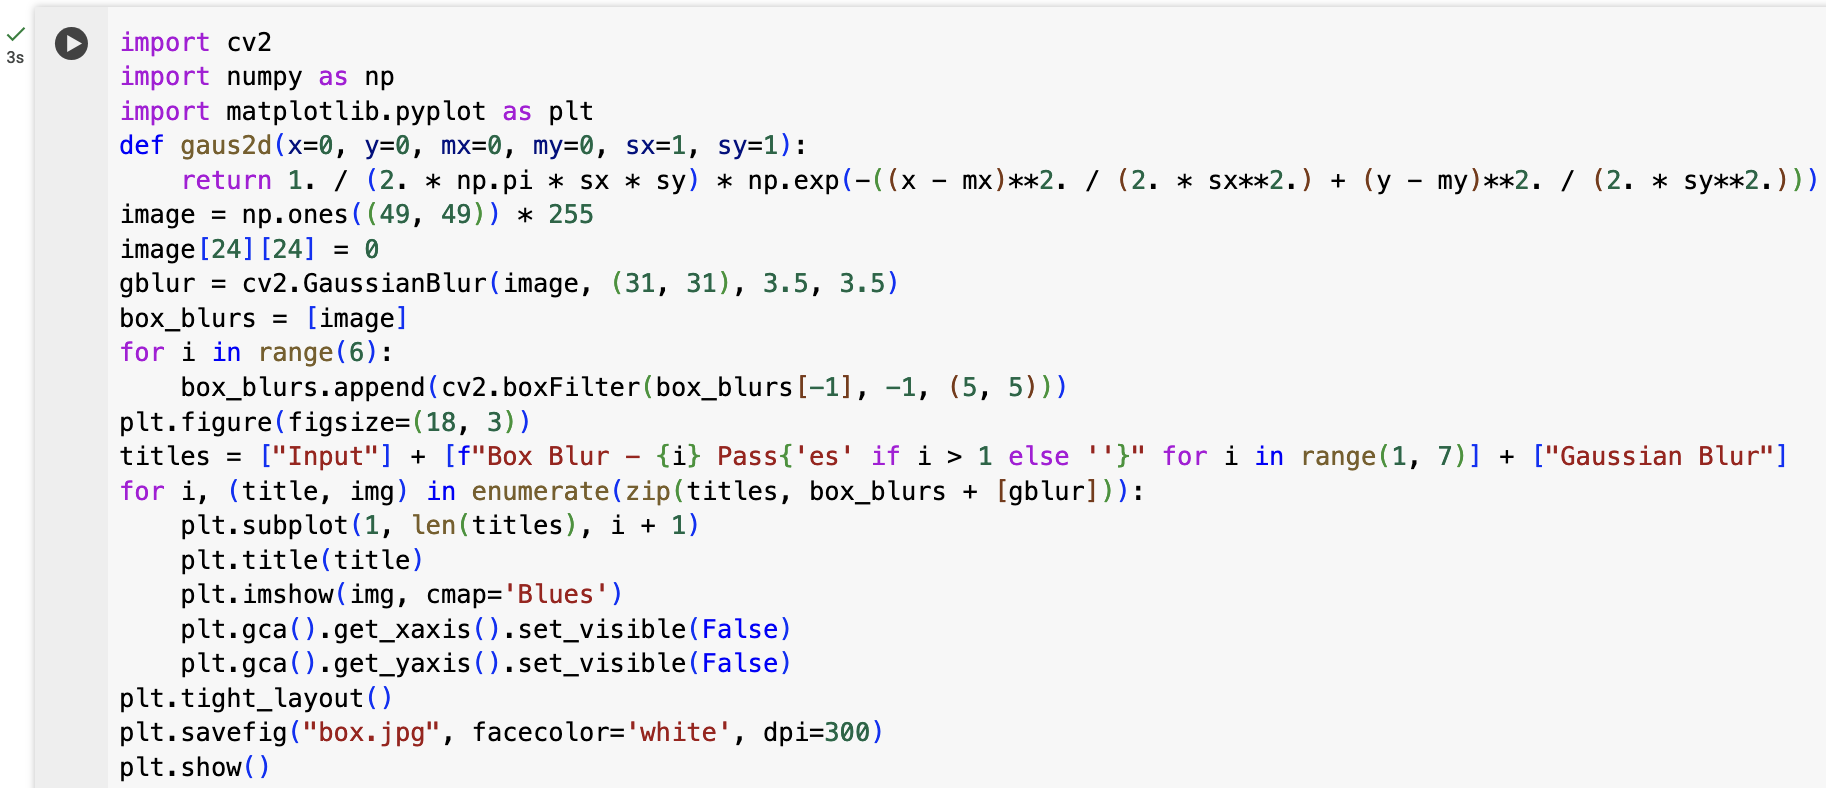
\includegraphics[width=1\linewidth]{figures/proofcode.png}
    \caption{Python code that displays the repeated box blurs after each iteration, in addition to the Gaussian blur.}
    \label{fig:enter-label}
\end{figure}

\end{frame}

\section{Future Work}
\begin{frame} {Future Work}
Future work would most likely involve the implementation of an algorithm to sharpen images using Laplacian of Gaussian.
\begin{block} {Laplacian of Gaussian (LoG)}
    We apply the Laplacian operator directly to the Gaussian kernel, resulting in the following equation:
$$
LoG(x, y) = \Delta \left( G(x, y) * I(x, y) \right)
$$
    Then, we expand this with full equations to:
$$
\Delta G(x, y) = \left(\frac{x^2 + y^2 - 2\sigma^2}{\sigma^4}\right) \cdot \frac{1}{2 \pi \sigma^2} \exp\left(-\frac{x^2 + y^2}{2\sigma^2}\right)
$$
This equation lends itself to edge detection, as the Laplacian blurring function may selectively blur non-edges, while the Gaussian smooths out noise, resulting in edge-detection with LoG. 
\end{block}
\end{frame}

\section{Applications}
\begin{frame} {Convolutional Neural Networks (ConvNet)}
\begin{figure}
    \centering
    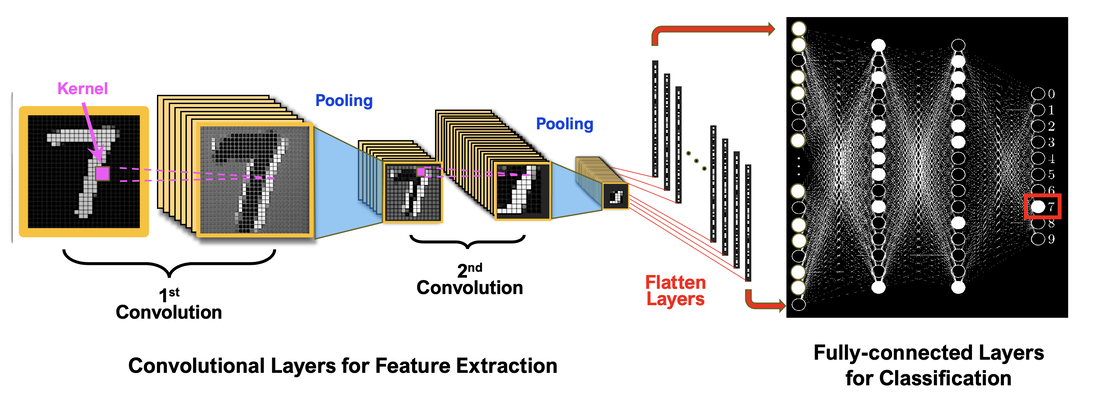
\includegraphics[width=1\linewidth]{figures/convnet.png}
    \label{convnet}
\end{figure}


\end{frame}
%---------------------------------------------------------
\section{Thanks!}
\begin{frame}{Thanks for Listening}
\begin{itemize}
    \item All information for implementation of our algorithm may be found here: \url{https://github.com/evankxiang/ssalinalgfinal}
    \item We have included CSV files of the image convolution algorithm and all raw code for the algorithm (.mat files). Furthermore, we include our old test files, primarily consisting of non-selective image blurring (no ability to select a bounding box). Finally, we include a preliminary sharpening algorithm using LoG that is a WIP. 
    \item EX, VP completed the programming segment. EX, RK, BB completed the slideshow and testing of the algorithms. Note, we are NOT listed in order of contribution.
\end{itemize}
\end{frame}

\end{document}